%
% $Id: ch02_relatedwork
%
%   *******************************************************************
%   * SEE THE MAIN FILE "AllegThesis.tex" FOR MORE INFORMATION.       *
%   *******************************************************************
\chapter{Related Work}\label{ch:relatedwork}

Genetic algorithms have been used to solve optimization problems for new buildings as well as for refurbished buildings. While some studies have focused on energy efficiency, others have included other factors such as material selection and structural design  \cite{Castro-Lacouture2009} \cite{Behboudi2012}. In this chapter, I will analyze five different studies involving building optimization using genetic algorithms as outlined in Table \ref{table:lit_review} These five studies have significant differences in their goals and depth, thereby providing a broad overview of the topic. I will mainly concentrate on how the authors formulated the objective functions, what variables they used in the genetic algorithm, and how they implemented their system.

\begin{table}[h]
\caption{Overview of the five studies reviewed in this chapter}
\centering
\begin{tabular}{|l|l|l|}
\hline
Author          & Year & Study Focus                                                                                                           \\ \hline
Magnier et al.  & 2010 & \begin{tabular}[c]{@{}c@{}}Thermal comfort and energy usage optimization \\ using GA and neural networks\end{tabular} \\ \hline
Milajic et al.  & 2013 & \begin{tabular}[c]{@{}c@{}}Methodology for green building design \\ using Multi-objective GA\end{tabular}             \\ \hline
Pejicic et al.  & 2012 & \begin{tabular}[c]{@{}c@{}}Optimal energy efficient building design \\ using GA and Tabu search\end{tabular}          \\ \hline
Pernodet et al. & 2009 & GAs for building refurbishment optimization                                                                           \\ \hline
Wang et al.     & 2005 & \begin{tabular}[c]{@{}c@{}}Object Orient Framework for building energy \\ usage optimization\end{tabular}             \\ \hline
\end{tabular}
\label{table:lit_review}
\end{table}

\section{Objective Functions}\label{sec:functions}

Wang et al. present a case study that uses their multi-objective framework to design a single story office building in Montreal, Canada \cite{Wang2005b}. The objective functions they use are the total life cycle cost and life cycle environmental impact for a green building design. They use exergy, i.e., the maximum theoretical work that can be done by a system with respect to its environment, as the indicator for environmental impacts \cite{Wang2005b}. Besides the exergy consumed by the building during its life cycle, they also consider the exergy required to remove or recover the wastes produced in the different life cycle phases of the building such as greenhouse gases \cite{Wang2005b}. For the cost objective, they consider the initial construction cost, the operation cost, and the pre-operation cost including resource extraction, transportation, etc. \cite{Wang2005b}. 

Milajec et al. use similar objective functions as Wang et al. i.e. life cycle cost and life cycle environmental impact. While they do include both cost of construction and of operation, they do not specify whether they include pre-construction cost as well. Their life cycle environmental impact assessment cost includes the cumulative exergy (like Wang et al.) but not the exergy required for waste recovery or removal. The Pernodet et al. study uses some similar objective functions as well. The main difference is that instead of two they use three objective functions \textemdash yearly energy consumption of the building in KwH/m\textsuperscript{2}, investment cost related to the refurbishment of the building, and an economic global cost defined as the ``sum of initial investment cost, the yearly energy cost and the yearly maintenance cost'' \cite{Pernodet2009}. Their study looks at optimizing the refurbishment of a school building in France.

Unlike the above studies, Magnier et al. and Pejicic et al. do not use cost as an objective function. Magnier et al. focus on thermal comfort as an objective function aside from energy consumption. Pejicic et al. use a case study to demonstrate multi objective optimization using a model single floor commercial building. Their goal is the optimization of insulation materials and orientation angle of a given building. 


\section{Building variables}\label{sec:variables}

Pejicic et al consider three building variables in their studies \textemdash building orientation, and inner and outer insulation materials from a set of ten different materials. Pernodet et al. \cite{Pernodet2009} focus on the building envelope parameters for their objective function. These include thermal transmittance of the walls and windows, glazing ratio and solar factor, air tightness of building envelope, and artificial lighting power. Similarly, Milajec et al. mainly consider structural variables as well incluidng wall, floor, and roof type and layers, building shape, orientation and structure. The Wang et al. study is much more in depth as they consider the most variables out of any of the above studies. Further, many of their variables are composed of other sub-variables. For instance, they have two different wall types and each wall type has a sub-variable called insulation among other ones. Insulation is a discrete variable that can take many different values, each corresponding to a different insulation material. Each wall type has a specific set of insulation materials to choose from. Besides wall type, Wang et al. look at floor types, roof type, and building shape. Each of these has its own set of sub-variables making the Wang study significantly more complex than the others. While the above studies consider only variables related to the building envelope, Magnier et al. use HVAC system-related variables in addition to the building envelope ones. They use a total of 20 different variables including heating and cooling set points, relative humidity set point, supply air flow rates, thermostat delays, window sizes, thickness of wall etc. The window sizes are separate for each wall and the HVAC system related variables are considered separately for two different seasons in a year. 


\begin{figure}[htbp]
\centering
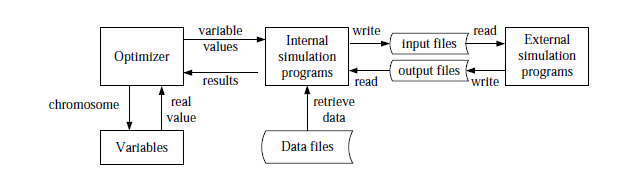
\includegraphics[width=\linewidth]{images/ooframework.png}
\caption{Object Oriented Framework used by Wang et al. \cite{Wang2005b}}
\label{fig:wang}
\end{figure}

\section{Implementation}\label{sec:implementation}
 Wang et al. \cite{Wang2005b} present an extensible object oriented framework implemented in C++ and Fortran (Fig. \ref{fig:wang}). The object oriented nature of the framework presented makes it easily extensible and promotes code reuse. The framework supports both continuous and discrete variables and implements algorithms to solve both unconstrained and constrained single objective optimization problems, but only unconstrained multi-objective optimization problems. Constrained, as the name suggests, limits the range of values for a variable to certain range as specified by the user while unconstrained does not. The framework integrates with the commercially available ASHRAE Toolkit energy simulator program and can be extended to integrate with {\em EnergyPlus}. The authors use the framework for a case study with impressive results and present a number of ways in which the project can be extended. While this framework can certainly be very useful as a starting base for my proposed project, it is not readily available as a open source project. 

Unlike Wang, other studies focus less on the software framework and more on the method of approach of completing the optimization process. Indeed, Pejicic et al. state that a ``solving methodology using evolutionary algoritms'' as their objective. A major difference in implentation between the Wang et al. study and the others is the energy simulation software used \textemdash both Milajec et al. and Pejicic et al. use EnergyPlus while Magnier et al. use TRYNSYS.  While TRYNSYS is widely used in industry (CITE), EnergyPlus is newer and cross-platform, and is freely available from the Department of Energy. In addition, it supports modelling a building through Sketchup through a free plugin. The ASHRAE Toolkit is older than EnergyPlus and does not support as many thermal modelling options either. Pernodet et al. do not use thermal simuation at all. Instead they estimate energy usage mathematically. This method is simple though it might be inaccurate for more complex buildings.

One of the main drawbacks of using an energy simulation program is that they are time consuming. Wang et al. report that a complete optimization run for their case study took about 70 hours. EnergyPlus and TRYNSYS would be even slower since their thermal simulation model is more complex. To counter this problem, Magnier et al. use an artificial neural netowrk (ANN) for fast evaluation. They use a multilayer feed-forward ANN to first mimic the behavior of the base building model, and then use this ANN inside the GA for fast evaluation of individuals (Fig. \ref{fig:magnier}). This technique is very efficient and reduces the computational time associated with each evaluation to almost negligible while maintaining a good accuracy \cite{Magnier2010}. The main limitation to this method is that the ANN needs to be trained before it can be used for the evaluations. The training period can take a relatively large amount of time. For instance, the training period in the Magnier et al. study was around 3 weeks. The advantage, however, is that the once the ANN is trained, it can be used for multiple runs of the system. A different approach would be to use a distributed model of computing by dividing the task of evaluating the fitness of an individual among a cluster of computers instead of a single one. While this method has not been used for optimizing building design in particular, it has been used for other similar multi-objective optimizaton problems. 


\begin{figure}[htbp]
\centering
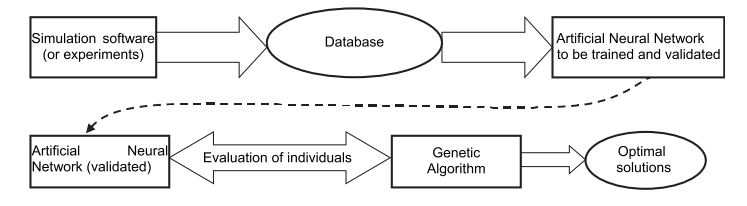
\includegraphics[width = \linewidth]{images/magnier.png}
\caption{Optimization system used by Magnier et al. \cite{Magnier2010}}
\label{fig:magnier}
\end{figure}



